\documentclass[11pt,twoside]{article}
\usepackage{natbib}
\usepackage{amssymb}
\usepackage{amsmath}
\usepackage{amsthm}
%\usepackage{fullpage}  % margins are a little *too* small
%
%  find the package that exports \setmarginsrb
%  and use it
%
\usepackage{setspace}
\usepackage{graphicx}
\usepackage{array}
\usepackage{tabularx}
\usepackage{verbatim}

\newcommand\dnr{\mathit{DNR}}
\newcommand\fail{\mathit{FAIL}}
\newcommand\pass{\mathit{PASS}}


\let\cite=\citep
\bibpunct();A{},

\title{Improved Ranking through Black Box Testing}
\author{Jesse Welch}
\date{May 2012}

\pagestyle{headings}

\begin{document}

\baselineskip=1.3\baselineskip % a little extra space between lines

\maketitle

\tableofcontents
\newpage

\section{Introduction}
Black-box testing is a useful method for diagnosing faults within a program. Rather than having to read through source code to find flaws, black-box testing allows a set of failures to be presented without any detailed knowledge required.

When a set of black-box tests are run on multiple solutions to a single problem, more information is available. Not only do we have the test results, but we have an ability to compare the test results. We can use this ability to find redundant tests, and limit the amount of noise shown for each solution. We can also use this information to compare the solutions, ranking them based on functional correctness.

Prior work demonstrates methods for both ranking and reducing redundant tests. In this paper, we will improve upon these methods in several ways. We will demonstrate a method for improving the ranking function by allowing additional results. We will introduce a method for allowing the ranking algorithm to continue to function with incomplete results. We will introduce a novel algorithm for performing additional noise reduction on each individual solution. Finally, we will introduce an infrastructure designed to make further algorithmic improvements and reduction strategies simple to implement.

\section{Ranking Solutions}
\subsection{What is Ranking?}
When we have multiple solutions to the same problem, we are generally trying to compare them in some way. Prior work has needed to compare various programming methodologies \cite{Claessen}. We have multiple outcomes because we are attempting to grade student homework assignments. The ability to compare the functional correctness of each submission helps us to group students into grade ranges and insure fairness in the grading.

"Fairness" is a particularly difficult concept to quantify, but it a fair ranking algorithm is necessary to be able to accurately compare solutions. A fair algorithm produces an objective comparison, in which the two solutions are correctly ordered by their functional correctness, regardless of the actions of an adversarial tester.

A ranking algorithm can therefore be improved by making it more fair. This can mean any of several things. If a new algorithm is able to find an objective relationship between two types of solutions considered equivalent by the original algorithm, the new algorithm is an improvement. Similarly, if a new algorithm discovers that two solutions are incomparable when the original algorithm found a relationship between them, the new algorithm is an improvement, because it has removed a relationship that did not truly exist.

Finding a fair ranking algorithm is exceedingly important for our task of grading student homework. Prior to implementing the algorithms below, our students were given feedback that listed their result on every test in our test sets, which were generally to large to be easily comprehended. Additionally, raw percentage of tests passed is not a fair metric by our definition. Consider two solutions, one with a bug in feature $F_1$, the other with a bug in $F_2$. An adversarial tester could easily choose which solution ranked superior by altering the number of tests run on each feature. If more tests are run on $F_1$, $F_2$ will be superior. If more tests are run on $F_2$, $F_1$ will be superior. Until we found an alternate algorithm, students could not be fairly compared algorithmically, and needed to be ranked based on the instructor's expert knowledge.

\subsection{The Algorithm}
Claessen et. al. demonstrated an algorithm for creating a fair ranking of solutions\cite{Claessen}. Their algorithm was run on large test suites generated automatically using QuickCheck \cite{QuickCheck}, which produces many similar test cases. In order to limit the number of tests they needed to consider, they partitioned the test set into equivalence classes.

\centerline{Given tests $T_O$ and $T_1$ and solution set $S$}
$$ T_0 \equiv T_1 \iff \forall s \in S : s(T_0) \equiv s(T_1) $$

Using this example, a test set $T$ could be reduced into a set of its equivalence classes. From these equivalence classes, a single representative example could be drawn, creating a new test set $T'$. $T'$ is a simpler set to work with than $T$, and processing it will be cheaper due to its decreased size. Most importantly, because $T'$ contains a test equivalent to every test in $T - T'$, the reduction has not lost any information.

%TODO: Proof by contradiction of this

Claessen's algorithm then creates a partial order of the solutions using $T'$. It does this using a binary representation of results. Tests can either be passed or failed, and PASS $>$ FAIL.

\centerline{Given solutions $S_1$ and $S_2$, and test set $T$}
$$S_1 \equiv S_2 \iff \forall t \in T : S_1(t) = S_2(t)$$
$$S_1 \sqsubseteq S_2 \iff \forall t \in T' : S_1(t) \geq S_2(t)$$


Under this definition, there are 4 possible results for comparing two solutions, $S_1$ and $S_2$. $S_1 < S_2$, $S_1 > S_2$, $S_1 \equiv S_2$, or $S_1$ and $S_2$  are incomparable. This definition allows us to build a partial ordering. This ranking is not built on the number of failures, but only on the direct relationships between the set of tests failed by each solution.

Using this algorithm, we are able to successfully create fair rankings of different student solutions.

\begin{figure}
\centering
\includegraphics{rank1.ps}
\caption{An edge points from a functionally inferior solution to a functionally superior one. "$\vert$" represents a class of tests passed by the equivalence class, "." represents a class of tests failed by the equivalence class.}
\end{figure}


\subsection{Adding More Outcomes}
The Claessen algorithm is based upon property based testing, for which the only possible outcomes are PASS and FAIL. Other forms of testing produce more outcomes. A solution can produce the right output, produce the wrong output, throw an exception, have a fatal error, or fail to terminate in a reasonable amount of time, among other possible outcomes.

Claessen's definitions already allow for non-binary outcomes. We need not change anything except what $>$ means. This step, however, presents an interesting problem. When allowing only binary outcomes, the total order of outcomes is self-evident: PASS$>$FAIL. When dealing with non-binary outcomes, however, there is no readily available ordering. Is an error that crashes the process ``better'' than one that silently produces wrong answers? In some cases, the process should be kept running at all costs. In others, the increased visibility of a catastrophic failure may be preferred to the subtle incorrectness of a wrong answer. In truth, the ranking of these outcomes is an arbitrary decision.

Since no universally correct ranking of outcomes is possible, we chose to examine what would happen if the algorithm was extended by a ranking determined by arbitrary choice. Though many orders could have been tried, for experimental purposes, we imposed a single simple arbitrary order. PASS$>$INCORRECT$>$FAILURE, where FAILURE is defined as an error that brings down the process/interpreter. We chose this ordering because our datasets represent student solutions, and the students were told that a segmentation fault (or related fatal error) would result in a 0\% as their grade on functional correctness.


\begin{figure}
\centering
\includegraphics[scale=0.75]{rank1.ps}
\caption{Created using binary outcomes}
\includegraphics[scale=0.75]{rank2.ps}
\caption{Created using multiple outcomes}
\end{figure}

Using our new comparison function (but an algorithm unaltered from Claessen's), we found several interesting properties. First, as demonstrated in Figures 2 and 3, in many cases, the additional outcomes made no difference. This was a surprising fact, and shows that the equivalence classes produced by the algorithm demonstrate a stronger degree of relatedness than previously known. Not only are these solutions getting the same binary results for every test, they are, in many cases, failing in  identical ways. Equivalence classes of solutions generally document programs that are \emph{extremely} similar.

In a small subset of our test cases
%TODO: quantify
we were able to improve the ranking using multiple outcomes. In most of these cases, it rendered incomparable solutions previously considered equivalent. This was due to them failing on the same tests, but in varying ways. In rare cases, we were able to rank solutions previously considered equivalent, generally because the solutions were identical, except on a subset of test on which one segfaulted and the other produced invalid output.

\subsection{Running Less Tests}

The computational power required to test a program adequately can be substantial. To fully exercise even a medium-scale program, thousands of unit tests (potentially generated from hundred of QuickCheck properties) may be required. Some or all of these tests may be expensive to run. A test that induces an infinite loop will run until an arbitrarily long timeout point. A test that does not induce an infinite loop may simply take a long time to run, or allocate large blocks of memory.

Running a test set can therefore be very expensive, particularly upon many solutions. Each expensive test needs to be run for each solution, and a particularly poor solution may cause many tests to loop infinitely. It would therefore be useful to not run the entire test set on every solution. 

For some of our test sets, we found that block testing was necessary for computational efficiency. For one of our assignments, we needed to test code in an interpreted environment. If we could not run tests in block, we needed to spawn an interpreter for each test. A test set created in this manner required ~4 hours of CPU time to run. Because test sets need to be debugged, this cost became prohibitively expensive.

Block testing, however, created its own set of problems. Rather than spawning a process for each test, we spawned a process for each block of related tests. If any of these tests brought down the entire process, results for any tests which were not yet reported were simply not reported. Instead, they received a new, implicit outcome: Did Not Run (DNR). Note that DNR means specifically that a test was not run at all. An outcome such as Did Not Finish (DNF) would appear explicitly in the test set.

With these new outcomes ``in'' our dataset, we were faced with the challenge of ranking based on them. There were two possible paths for ranking these solutions. The first would be to simply use the process described in the previous section, and extend the comparison function to place DNR arbitrarily within the ordering (perhaps as the worst result, or equivalent to a fatal error). This solution is simple, and allows us to reuse the modifications above. However, by giving DNR a place in the ordering, we limit what can cause a test to not run.

The tester running the test set may choose to omit tests from a given solution for any number of reasons. Perhaps tests are omitted for the reasons we used, because a previous test caused a fatal error. But perhaps thy are omitted for a more positive reason. A tester could choose to start a portion of a test set by running an extremely difficult test set, one which simultaneously exercised every feature that portion is testing. If this test is passed, they may then choose to not run all of the simpler test cases, because they know the solution will pass them. And perhaps the tester eliminates some tests for each of these reasons, on the same test. In this case, there is no proper place for DNR in the ordering of outcomes. It could mean either PASS or FAIL, and so cannot be placed as better, worse, or equivalent to any of them.

In this case, we can choose another method for handling DNR outcomes. The procedure is very simple.

\centerline{Given solutions $S_1$ and $S_2$, and test set $T$}
$$S_1 \equiv S_2 \iff \forall t \in T where S_1(t) \neq \dnr \wedge S_2(t) \neq dnr \wedge S_1(t) \equiv S_2(t)$$
$$S_1 > S_2 \iff \forall t \in T where S_1(t) \neq \dnr \wedge S_2(t) \neq dnr : S_1(t) \geq S_2(t)$$
In this way, we do not invalidate any of the possible meanings of DNR. In a properly formed test set, two solutions cannot differ only on tests for which one of them received a DNR. Instead, a prior test result must have \emph{caused} the DNR in one solution and not the other, and on this test they can still be compared. 

In the first situation previously discussed, in which a block of tests may not be run because a prior test crashed the block, solutions would differ on whether or not they ran the block, but the one which ran the block would also have an inherently better result---it passed the test which crashed the block. The solutions can be properly compared on this test.

In the second situation previously discussed, in wehich a block of tests may not be run because a prior test had a successful result, solutions would differ on whether they ran the block, but also on the initial test---the solution which did not run the block has an inherently better result---it passed the test which caused the block to not run. The solutions can be compared on this test.

Using this process, solutions can be compared whenever tests are not run, for whatever reason they are not run, as long as the reasons are deterministic. If tests are not run for a reason, we can still compare the solutions, based solely on the reason, \emph{without information loss}.

\section{The Implication Graph}
\subsection{Finding Relationships}
The methods described above treat each test as a distinct entity. They are used to compare solutions, but they are never compared to each other, and are treated as if they were independent. In real test sets, there are frequently subset of the tests which are not independent, but which instead build upon each other.

An example of this occurred when we tested student solutions to the problem of reducing terms in the lambda calculus. One feature we tested was whether students had properly implemented $\eta$-reduction. To test this, we enumerated terms with "holes" in them, and placed a subterm that should be eta-reduced within the hole. Two terms created are: 
$$T_1 : \lambda a.M_\eta a$$
$$T_2 : \lambda x.\lambda x.\lambda a.M_\eta a$$
$T_1$ tested an $\eta$-reduction on its own, with no other variables. We hypothesized that, if a student was to correctly reduce any other terms containing $\eta$-reductions, such as $T_2$, they would need to be able to successfully reduce $T_1$.

If our hypothesis is correct, there should be an underlying relationship in the data set. Failing $T_1$ should imply failing $T_2$. Additionally, failing $T_1$ should imply failing every other test that contains an $\eta$-reduction.

This hypothesis was known beforehand. However, the dataset contains many relationships similar to this implication. We have classified these relationships into four categories: real implications, accidental implications, trivial implications, and bogus implications. Real implications are those such as $T-1 \Rightarrow T_2$ above, which document an actual relationship between tests. Accidental implications are those which are represented in the data, but which have no bearing on the outer world, and are instead an "accident" of the solution population. Trivial implications include tautological implications and implications incidentally caused by a small piece of data, which are not representative of the entire solution population. Bogus relationships are those which are defined within the data, but which, given a sufficiently large population of solutions, could not possibly exist.

We create a structure we call the implication graph, which documents these implications. The simple implication graph includes every implication from all four classes. An improved implication graph attempts to eliminate as many trivial, bogus, and accidental implications as possible, while retaining the real implications.

\subsection{Creating the Graph}
An implication is defined as follows:

\centerline{Given solution set $S$ and outcomes $O_1$ on test $T_1$ and $O_2$ on test $T_2$}
$$O_1 \Rightarrow O_2 \iff \forall s \in S where s(T_1) = O_1, s(T_2) = O_2$$

Using this definition, we attempt to discover every implication in the dataset. First we create a proposition for every outcome, and its inverse, on every test. Then we look for an implication (in either direction) between each pair of propositions. This is a $O(n^2)$ process, but by limiting computation to one test from each equivalence class of tests, n remains small enough to proceed.

This process is simplified even further by usage of a variation of the partitioning algorithm used to create the equivalence classes of tests. Rather than partitioning the tests, we partition the \emph{propositions} into equivalence classes. For a given solution, a proposition is considered true if it holds on that solution (e.g. the proposition Test 2 PASS hold for a solution if it passes Test 2), and false if it does not hold. Two propositions, $P_1$ and $P_2$, are considered equivalent if they hold for the exact same set of solutions.
$$P_1 \equiv P_2 \iff \forall s \in S, P_1(s) = P_2(s)$$
Now, rather than having to find implications between every proposition, we need to find them between every \emph{class} of propositions.

The set of implications within a dataset forms a natural structure: a directed graph. Each class of propositions is a node in the graph, and each implication is an edge from the implicating proposition to the implied.

\begin{figure}
\verbatiminput{toyimpldata}
\includegraphics[scale=0.75]{toyimpl.ps}
\caption{Dataset and the generated implication graph. A transitive reduction has been performed on the graph}
\end{figure}

Given this implication graph, the question remains: How many of the implications in the graph are real implications? We were provided with a natural experiment to begin to test this question. Our students were given an assignment that contained 14 problems. Each of the problems was entirely self-contained, and there was no code overlap between the problems. Some problems covered related topics, and so relic relationships might appear in the data, but by and large, we expected these problems to be diagrammed as entirely separate components.

\begin{figure}
\includegraphics[scale=0.5]{div.ps}
\caption{Implication graph generated from experiment. Boxed sections indicate tests performed on the same problem. TODO: ADD BOXES}
\end{figure}

The results of this experiment were mixed. We did not find that every subproblem made an entirely separate subgraph, but instead that the subproblems made subgraphs that were sometimes connected, with implications between portions of the problem that should not be possible in the underlying problem.

\begin{comment}
\subsection{Improving the Visualization}
The implication graph, as produced contains all of the information about implications contained within the dataset. It also contains large amounts of tautological information, implications which are true regardless of the dataset. These tautologies are represented both as edges within the graph and as equivalences within a single node.

These tautologies are generally relationships between propositions that work on the same test. If a test $t$ fails, $t$ did not pass; if $t$ does not run, $t$ did not fail, etc. Informing the person analyzing the implication graph of these relationships adds nothing to the structure of the problem, it merely dilutes the relevant relationships. Though removing these tautologies removes information from the graph, it is not information that an intelligent viewer will not readily assume.

There are two processes necessary for removing tautologies from the implication graph, one if they are within a single node, another if they are between nodes. Removing an intranode tautology is simple. One of the two tautologically propositions is simply removed from the node, leaving only one member of the pair. In our implementation, we attempted to retain the more precise proposition (PASS is more precise than NOT FAIL, because it describes only one outcome and not a set). 

Removing internode tautologies is equally simple, though more likely to confuse the viewer. Any of the relationships between two equivalence classes of propositions is tautological, we remove the edge in the graph. This relationship can still be assumed by an intelligent viewer, because the tautology remains self evident. However, the relationships between the other members of the equivalence classes have now become implicitly documented, rather than explicitly.

Also present in the implication graph is an entire class of redundant relationships. For two related propositions, $A$ and $B$, two implications are created: $A \Rightarrow B$ and $\neg B \Rightarrow \neg A$. This is true for two equivalence classes as well, the negation of a class being the negation of each of its members. Given one of these implications, the existence of the other is tautological. Therefore, we can include only one of them, without suffering information loss to an intelligent viewer. A difficulty in implementation lies in choosing a subset of these implications that leaves a minimal number of nodes in the final graph.

Intelligent viewers may choose whether or not performing any of these reductions on the implication graph increases clarity by limiting the amount of information displayed, or reduces clarity by rendering some relationships implicit. Nonetheless, it is clear that performing these reductions causes a substantial reduction to the size of the resulting implication graph.

\begin{figure}
\includegraphics[scale=0.5]{div.ps}
\newline
\includegraphics[scale=0.5]{divreduced.ps}
\caption{The previous experimental graph before and after reduction. Note the significant decrease in both the numbers of nodes and edges between the graphs.}
\end{figure}
\end{comment}

\section{Noise Reduction}

\subsection{What is Noise?}
A piece of data is classified as noise if it can be removed without causing any loss of information. For example, in Figure {?} we show that the number of tests run is generally far greater than the number of equivalence classes they form. However, for our ranking algorithm, we only need a single representative from each equivalence class to create our ranking. The non-representative members of each equivalence class are noise. 

Noise can be found in any section of a data set. It can be entire tests, as above, or single outcomes. In either case, its presence in the final output of our program is a negative force. The more noise there is in the final data, the less likely it is for the reader, in our case a student, to discover the useful information.

For this reason, we seek to reduce noise as much as possible. Ideal noise reduction algorithms would provide each student the minimum subset of testing data required to accurately compare themself with other students, and properly diagnose the faults within their program.


\subsection{Claessen's Algorithm}
In Claessen's paper on ranking, there are several forms of noise reduction already performed. The first is the fundamental step of the algorithm, in which tests are grouped into equivalence classes. This step alone reduces from the original number of tests to a substantially smaller subset. Even with test sets numbering well into the thousands, this step never produced more than 144 equivalence classes during our experimentation.

After this large scale reduction, Claessen's algorithm contains another form of noise reduction. A test $T_0$ is redundant if

$$\fail (T_0) \equiv fail(T_1) \cup \fail(T_2)$$
where all three tests are drawn from different equivalence classes. This was justified with the argument that, rather than discovering a new faults of its own, $T_0$ likely provoked both of the faults discovered in $T_1$ and $T_2$. Removing $T_0$ therefore does not cause any information loss. Instead, its removal simplifies the test set to a smaller, but still representative sample of tests.

\subsection{Union*}
The logical basis to Claessen's algorithm that a test can be redundant because it provokes the flaws already demonstrated by two other non-redundant tests\cite{Claessen}, can be extended further. Why should we limit this to only circumstances where the flaws are in exactly two other tests? Why not any number? We propose an extended algorithm, one which removes any tests whose set of failures is equal to the union of the failures of \emph{any number of tests}. 

A test $T_0$ is redundant if

$$\fail (T_0) \equiv \fail(T_1) \cup \fail(T_2) \cup ... \cup \fail(T_n) $$

(if I managed to write the first proof, proving this the same shouldn't be hard)

A naive implementation of this algorithm is computationally complex. Given a set of tests $T$, we need to run the algorithm for each member $t$ of $T$, checking whether its failure set is equal to the union of any subset of tests in $T$ that does not contain $t$. This is simply too much work, so a different solution must be found.

Thankfully, the implication graph lends itself to a vastly simplified implementation. We do not need to check the union of every possible subset of tests, only the union of those that could possibly be useful. Using the implication graph, given a test $t$ and a test set $T$, we can easily find the subset $T'$ which only contains tests whose failures are a subset of $t$. Any test in $T$ but not in $T'$ cannot possibly contribute to an equal union, because it contains at least one failure not in $t$. Therefore, we can simply apply the algorithm once, to every member of $T'$. $t$ is redundant if $FAIL(t) \equiv \cup^* T'$.

\subsection{Comparison}
Union* must reduce at least as many tests as Claessen, and can reduce more. This is because every test that will be removed under Claessen will be removed under exactly the same conditions in Union* (the union of two tests is simply a specification of the union of any number of tests). In theory, Union* is capable of outperforming Claessen

\begin{figure}
\verbatiminput{testset}
\includegraphics{toy.ps}
\caption{Reduced under Claessen. t = {1,2,3,4}}
\includegraphics{toyb.ps}
\caption{Reduced under Union*. t = {1,2,3}}
\end{figure}

%TODO: Table with different levels of reductions. Then change the text below to handle whatever I put in the table.

In practice, we discovered a different situation. On 10 different real world datasets (each dataset was the student submissions for a different assignment, drawn from two different courses), we found no difference between reduction performed by the Claessen algorithm and the Union* algorithm. This was a surprising result, and demonstrates several things. Trivially, it confirms that the Union* algorithm does no worse than Claessen. More substantially, we discovered that the Claessen algorithm is surprisingly powerful. In every tested real world case, the union of two tests was enough to remove every test that could be found redundant under union.

There are several potential explanations for this fact. One is that no test tests more than two underlying faults. This is extremely unlikely, as it is relatively simple to write a test that exercises large sections of a program's functionality, and can readily provoke more than two potential faults. Another possibility lies in the method of building tests. When unit tests are written, they generally exercise small areas of functionality, rather than the entire program. A different style of test design might allow Union* to have more success, removing large tests that attempt to exercise every possible fault in the program, when these faults are better demonstrated by small tests. A final possibility is that we simply don't have enough solutions, and that a greater diversity in solutions would increase the difference between the two algorithms.

\subsection{Improving the Implication Graph}



When building the implication graph, we do not have access to the structure of the problem itself, only a small sample of attempts to solve the problem and there results on tests of the problem. We have no oracle to tell us when the structure is correct. However, there are many properties about the relationships between tests that we can utilize to remove implications that cannot possibly be present in the problem itself, as well as removing implications that may be true, but the we do not have enough information  to claim.

One class of implications we can remove entirely are those between the failure of one test, and the passage of another. Every problem has a fully correct and a fully incorrect solution, one which passes every test, and one which fails every test. Based on this, the following proofs are possible.


Assumption: There exists a fully correct and fully incorrect solution to every problem.

Theorem: The passage of one test cannot imply the failure of another test in the full problem space.

Proof: Assume $PASS(T_1) \Rightarrow FAIL(T_2)$. This means that every solution that passes $T_1$ fails $T_2$. However, there exists the fully correct solution S. For all tests T, S(T) = PASS. Therefore S($T_1$) = PASS, and S($T_2$) = PASS, contradicting our assumption.

Theorem: The failure of one test cannot imply the failure of another test in the full problem space.

Proof: Assume FAIL($T_1$) $\Rightarrow$ PASS($T_2$). This means that every solution that fails $T_1$ passess $T_2$. However, there exists the fully incorrect solution S'. For all tests T, S'(T) = FAIL. Therefore S'($T_1$) = FAIL, and S'($T_2$) = FAIL, contradicting our assumption.


Based on these proofs, we can safely remove from the implication graph every implication between the passage of one test and the failure of another.

From similar logic, we can remove every implication either to or from a test with universal results. If every student passed a given test, then any result on any other test will logically imply this passage. However, there exists the fully incorrect solution, which by definition failed this test. Therefore these implications are by definition based on incomplete information, because they do not take into account the failure of this test. The inverse means we can do the same to a test which every student failed, based on the fully correct solution. Similarly, if no student passed a given test, the  test's passage will logically imply everything. But we cannot make implications  from this result (or a test with no failures) because the fully correct and incorrect solutions mean we are basing these implications on incomplete data.

There is one other reduction we can make to the implication graph, for somewhat different reasons than the previous reductions. We can remove implications that may hold true in th actual problem structure, because we do not currently have enough information to assume them. If a given test result is achieved only by members of a single equivalence class, any implications based on it can be removed, because they are based on too little information to generalize from.

We don't have enough information because, if an outcome is achieved only by a single class, it logically must imply every other result achieved by that class's solutions (because every solution that achieved that result achieved each other result). But we simply cannot claim that each of these results is directly implied by a single result. If we do, we claim that knowing a single fact about a solution means that we know everything about it. This is obviously untrue.


\section{Reducing Noise in Witness Sets}
\subsection{Witness Sets}
When grading students, successfully ranking them is not the only goal of creating and running a test set. An additional goal is providing the student with feedback on the flaws within their program. We do this programmatically by providing them their test results on each test which they failed, as well as a witness describing what went wrong.

This witness set is drawn only from the tests which are used to rank the student solutions. Thus, the noise reduction strategies above implicitly reduce noise in the witness set, by eliminating tests from consideration. However, this still leaves many tests in the witness set, and we believe many of them can be classified as noise. If this noise can be reduced, students can be provided a simpler set of witnesses, making it easier for them to understand the flaws in their programs.

\subsection{The Algorithm}
Any reductions that can be made on the basis of classes of solutions will already be implemented as reductions within the ranking graph. However, when attempting noise reduction at the granularity of a single solution, the relationships between solutions are not applicable. The only relationships relevant at this level  are those between the tests themselves.

The implication graph is a representation of the relationships between these tests. It presents many discoverable relationships (implies, implied by, reachable from, etc.). Using this graph, we are able to perform noise reduction at the level of a single solution, a novel process. For simplicity, we chose to examine only one of the available relationships, direct implication. Our algorithm is as follows:

\centerline{Given two tests $T_1$ and $T_2$ and solution $s$}
$$if s(T_1) = FAIL \wedge FAIL(T_1) \Rightarrow FAIL(T_2), remove T_2$$

Given a perfect implication graph, in which every implication is not just found in the data but representative of the problem itself, this algorithm reduces the tests presented as  failed to the set of the easiest tests failed. 

If two tests are needed to differentiate the solutions on the solution class scale, it is possible (and frequently true), that one is simply an easier version of itself. For example, take the lambda terms described above when creating the implication graph. 

$$T_1 : \lambda a.M_\eta a$$
$$T_2 : \lambda x.\lambda x.\lambda a.M_\eta a$$

Because the flaw in $T_1$ directly causes a failure in $T_2$, $FAIL(T_1) \Rightarrow FAIL(T_2)$. This led our algorithm to be able to reduce the witnesses to any solution who failed both tests, providing only the output from $T_1$.

\begin{figure}
\verbatiminput{lambdareduction}
\caption{Machine output for a successful reduction in which $T_2$ (nr403) was removed due to failure of $T_1$ (nr97)}
\end{figure}

\subsection{Validity of Reductions}

This algorithm is definitively  capable of performing reductions, but a questions remains: Are the reductions good? Reductions performed on the class level cannot change the class structure. Both the Claessen algorithm and the Union* algorithm cannot cause information loss. But the witness reductions can. Though implications have a theoretical underlyin structure, they are drawn from the underlying data available, and this data is frequently flawed. This can lead to reductions in a test can be removed based on an implication from a test which tested an entirely different separate feature.

A readily available example is the dataset used to confirm the implication graph. As we discovered earlier, when tests were run on functions whose implementations were entirely independent, the functions generally formed into groups in the  graph, but there were implications between the groups. Using this implication graph, we performed a witness reduction on each solution, in order to test how many of the reductions we considered to be valid. In order to simplify analysis, we did not try ot delve into the relationship between each test, but instead used a simple metric. If two tests test the same function, any reduction upon them is valid. If they test different  functions, any reduction on them is invalid.

%\begin{figure*}
%\begin{tabularx}{\linewidth}{@{}XX@{}}
%\small\verbatiminput{goodreductions}
%&
%\small\verbatiminput{badreductions}
%\\
%\caption{Good reductions}&
%\caption{Bad reductions}
%\\
%\end{tabularx}
%\end{figure*}

\begin{figure}
\verbatiminput{goodreductions}
\caption{Valid reductions.}
\verbatiminput{badreductions}
\caption{Invalid reductions.}
\end{figure}


After running this experiment, we found that the witness reduction strategy achieved moderate success. Out of 422 reductions, 62.5\% were deemed to be valid. However, this result is somewhat misleading. A large number of the invalid reductions were concentrated in the least correct solutions. By omitting the reductions obtained from the two least correct solutions, the percentage of correct reductions jumps to 76.7\%. While eliminating these students is not something that can truly be done in practice, it demonstrates that witness reduction is highly accurate for most students, and extremely inaccurate for a select few.

Using the same definition of implications, but with multiple outcomes, we found a very different result. There were only 112 reductions, all of them related to the qsort function, and every one of them was valid. This was a positive result, but the fact that reductions were not made on tests of any other functions makes these results suspect.

Any invalid reductions discovered represent a failure in the implication graph, as they are based on implications which are likely not valid to the problem itself, but simply to the dataset the reduction process was done on. If the implication graph perfectly represented the problem structure, every reduction based on it would be good. Therefore, the more correct we make the implication graph, the more correct we make the witness reduction.


\subsection{The Results  of Improving the Implication Graph}

These reductions of the implication graph were critical to our ability to implement witness reduction. The first several reductions insured we were not making any reductions based on clearly invalid implications. The final reduction, in which we do not allow implications based on unique outcomes, was particularly important. Based on this reduction, we were able to improve the output give larger and more representative witness sets to the affected solutions.

\begin{figure}
\verbatiminput{example.witness}
\caption{Unreduced output}
\verbatiminput{example3.witness}
\caption{Reduced with unreduced implication graph}
\verbatiminput{example2.witness}
\caption{Reduced using improved implication graph}
\caption{In the student's code, none of the functions call each other. Therefore the reduction across tests is not only invalid under our metric, but accidental based on the code base.}
\end{figure}

\subsection{Continuing Problems}

Despite these reductions, we were not able to fully stop the algorithm from making invalid reductions. Though the implication graph can assuredly be improved further, and the witness reductions therefore improved as well, it is unlikely that we will ever be able to make completely valid reductions for most problems. The reason for this is twofold: the number of solutions available is finite, and  real world solutions are strange.

The first problem is fairly clear. In order to find the full structure of a problem, we need to know every possible correct and incorrect solution to it, an infinite  number of solutions. Presented with a finite dataset, we can only approximate this structure, a fundamental limitation.

The second problem is far more insidious. When attempting to find the structure of a problem, it is expected that if a test tests some feature of a program, and that feature has a flaw, the test will uncover it. However, in the real world, programs do not behave nicely. There may be two flaws within a feature, which generally cause the feature to fail, but sometimes work together to cause it to succeed.

In real world programs, we do not find clean connections of components, failures that always occur in concert, features bein implemented in uniform ways. Real programmers have flaws present at every known edge case, and sometimes at edge cases that were unknown. Flaws interact in unexpected ways, and programs, when tested as a black-box, are generally unpredictable.

Nonetheless, we have found that, on real world datasets, witness reduction based on our best approximation of the implication graph is good enough to produce positive results. Though the eccentricities of real programs often meant that reductions the seemed obvious were not made, and sometimes that invalid reductions were, the process generally proved successful, and should prove more successful as future improvements to the graph are made.

\subsection{Witness Expansion}

The end goal of witness reduction is providing the smallest possible set of tests that diagnose the faults of a solution. A related goal is providing a solution the most accurate diagnostic information possible. The implication graph can be used to achieve this goal by expanding the witness set, rather than reducing it.

When we believed two tests were related based on the implication graph, we removed the harder test, because the simpler one provided the diagnostic information. However, for a more successful solution, which passed the easier test but failed the harder one, we provide no evidence of this relationship. But this relationship is a very useful thing, because it provides increased specificity on exactly where the fault lies within the solution. Using a very similar formula to our witness reduction, we can provide the student with these relationships.

\centerline{We inform a solution $S$ which passed test $T_1$ but failed $T_2$ of the results on  $T_1$ iff}
$$ S(T_1) = PASS \wedge S(T_2) = FAIL \wedge FAIL(T_1) \Rightarrow FAIL(T_2)$$



\section{Future Work}
This paper utilized the implication graph in order to implement several forms of noise reduction. These are not, however, every form of noise reduction the graph can be used for. By documenting the structure of a problem, the implication graph makes it easy for a researcher to implement new reduction algorithms. For example, rather than removing tests whose failures are the union of the implying failures, we could remove any test whose failures are the intersection of the implied failures. Or any test where every outcome is implied by another test. There are many possible reduction algorithms, and with the infrastructure of the implication graph in place, these algorithms can be readily implemented.

The implication graph's utility is not limited to noise reduction, or to problems in which ranking solutions is a goal. The implication graph diagrams the structure of a problem, and knowledge of this structure allows us to analyze other problems as well. This is particularly intriguing for problems in which a fully correct solution is unlikely, and quality is judged on accuracy, such as machine learning problems. Knowledge of the structure of this problem might allow a researcher to discover sets of difficult cases which fail together, or to better understand how the machine algorithm works.


\section{Conclusion}
There already exist in the literature algorithms to rank programs based on black-box testing results. These algorithms are successful, but they use only a subset of the information available. We have attempted to use as much of the information present as possible to improve the existing algorithms and create our own.

Our Union* algorithm uses more of the testing data available to build a generalization of the union based reduction strategy implemented in \cite{Claessen}. This strategy proved to have minimal effect on the number of reduced tests in practice, but is computationally simpler than the Claessen algorithm, once the infrastructure has been built.

Our witness reduction algorithm is an entirely novel form of noise reduction. Rather than reducing tests only for the entire set of solutions, this algorithm allows further reductions to take place for each individual solution, creating a smaller set of failed test cases from which the solution's creator can diagnose faults.

Most importantly, we have created a powerful infrastructure from which further methods of noise reduction can easily be implemented. Rather than having to redesign for each new algorithm implemented, the implication graph allows for new reduction algorithms to be quickly implemented, and for entirely new types of reductions to be tested.

\bibliographystyle{plainnat}
\bibliography{thesis}

\end{document}
